\documentclass{casicswhitepaper}

\newcommand{\totalrespondents}{69\xspace}
\newcommand{\totaldevelopers}{56\xspace}
\newcommand{\totalsearchers}{55\xspace}

\begin{document}
\title{How scientific software users choose what they use:\\
preliminary results from an empirical survey}
\date{\dateAndVersion}
\author{Matthew J. Graham and Michael Hucka\\
\mailto{mjg@caltech.edu},\quad\mailto{mhucka@caltech.edu}\\
California Institute of Technology\\
Pasadena, CA 91125, USA}
\maketitle

\begin{abstract}
When they seek software for a task, how do scientists go about finding it?  Past research and anecdotal evidence suggest that searching the web, asking colleagues and reading papers have been the predominant approaches---but is that still true today, given the increasing use of social media and socially-centric online systems such as Stack~Overflow and GitHub?  In addition, when they \emph{do} look for software, what are the main characteristics that influence scientific users' choice of software?  And finally, if a catalog of software were to be developed to help people find software, what kind of information would they like to see in it?  These are the questions that motivated a survey we conducted in late 2015.  The survey was designed to capture current practices and experiences in searching for software from two distinct groups: those looking for ready-to-run software and those looking for software source code.  We present the results of our survey and discuss our findings in this report.
\end{abstract}


\section{Introduction}

Despite that software is critical to most research~\citep{bauer2014exploratory, hettrick_2014, hannay_2009, baxter_2006, wilson_2006}, finding software suitable for a given purpose remains surprisingly difficult~\cite{cannata_2005, Bourne::2015, SoftwareDiscoveryIndex:2014}.  Few effective resources exist to help users discover alternatives or understand the differences between them.  The pervasiveness of the problem was made clear in a recent study of developers at Google; the authors found that the factor ``most disruptive to the [software] reuse process'' was ``difficulties in finding artifacts''~\cite{bauer2014exploratory}.  In other words, \emph{even the developers at Google have difficulty finding software}.

When asked, many people reply that they look for software by searching the web with a general-purpose search engine such as Google.  Despite its popularity, this approach suffers from significant problems: Web searches can yield dozens of viable candidates---and millions of irrelevant results.  Moreover, some questions cannot be answered through Web searches without substantial additional effort, such as what are the \emph{specific} characteristics of different software tools or how do tools \emph{differ} from each other.  Many scientists also turn to the scientific literature to learn what others have used for similar tasks or research domains.  Searching the literature can increase the relevance of results and provide other useful information, but it suffers from limitations too: publications are static documents that can take years to produce and may not reflect a tool's current capabilities~\cite{wren_2004}, and moreover, not all tools are mentioned in publications or have a publication associated with them.  (As an example, the recent article~\cite{abbott2016observation} announcing the first-ever detection of gravitational waves lacked any mention of any software used.)  This may be for various reasons, such as article page length limits or a disinclination on the part of researchers to describe their full software stack or workflow.  Still other potential methods for finding software include asking colleagues, asking on social media, searching scientific computing gateways, and more.

The difficulty of finding software and the lack of better resources brings the potential for duplication of work, reduced scientific reproducibility, and poor return on investment by funding agencies~\citep{cannata_2005}.  We are interested in developing better resources to help users, particularly scientific users, discover software.  In order to gain a better understanding of the factors that influence how software users locate software, we developed and distributed an electronic survey beginning in September, 2015, which we advertised to numerous mailing lists serving communities in astronomy and systems biology.  We report on our methods, the survey responses, and our analyses below.


\section{Survey design}

Our survey was designed to shed light on current practices and experiences in searching for software in two different situations: looking for ready-to-run software, and looking for software source code.  Respondents did not have to be software developers themselves (although the results show that most were).  We chose to use a Web-based survey because it is an approach that (1) is well-suited to gathering information quickly from a wide audience, (2) requires modest development effort, and (3) can produce data that can be analyzed qualitatively and quantitatively.


\subsection{Instrument development}

We developed the survey instrument iteratively.  We began with an initial version in which we posed many questions related to searching for software.  Following the practices of other similar surveys in computing~\cite[e.g.,][]{varnellsarjeant2015comparing}, we iterated on the design of the instrument, paying attention to the following points:

\begin{itemize}

\item Wording.  We sought to make the questions clear and unambiguous, and avoid implying a particular perspective.  We elaborated each question with explanatory text under the question itself.

\item Relevance to user's experiences.  We limited our questions to topics that could reasonably be assumed to be within the experiences of our audience.

\item Contemporary circumstances.  We tried to ground the questions by referring to real resources and specific software characteristics that we believe are relevant to computer users today.

\item Ethics.  We avoided questions that might be construed as being too personal or about proprietary policies at respondents' place of work.

\end{itemize}

To help iterate on the design of the survey instrument, we performed a pilot survey with close colleagues as subjects.  Based on their feedback, we removed or expanded questions as necessary to achieve the final version.  The final survey form is presented in Appendix~A.  The instrument contained a total of 22 questions (of which 18 were content questions), and included conditional branches so that the final number of questions actually seen by any given respondent depended on the answers selected to certain screening questions.  There were five main groups of questions in the survey:

\begin{enumerate}

\item Basic demographic and general information, suitable for all respondents.

\item Questions for software users who have the freedom to choose software.  This section was only shown if respondents indicated that they have some choice in the software they use.

\item Questions for software developers.  This section was only shown if respondents indicated that are engaged in software development.

\item Questions for software developers who search for source code.  This was only shown if respondents indicated both that they are software developers and that they search for software source code.

\item Survey feedback.  This section sought feedback about the survey itself.

\end{enumerate}

Questions in section No.~2 aimed to establish the relative importance of different search criteria.  Those in section Nos.~3 and~4 sought to characterize the experiences of the developer.

The survey form used a mixture of four types of questions: check boxes, pull-down selection menus, two-dimensional rating grids, and short-answer input fields.  Some of the questions allowed answers on a nominal scale (for example, approaches used for finding software), some questions used an ordinal scale (for example, the importance of different considerations when looking for software), and some were open-ended questions asking for free-form text.


\subsection{Sampling plan}

We used nonprobabilistic convenience sampling with self-selection.  We advertised the survey on mailing lists and social media oriented to the astronomical and biological sciences.    The number of potential participants is unknown, because we cannot track the redistribution of the survey invitation.  Consequently, the response rate is unknown.

Potential biasing factors in the results are the same as those common to most self-selected written surveys that use convenience sampling.  These include response bias (i.e., people who responded may have different characteristics than those who did not), coverage errors (i.e., the representation of respondents may not be balanced across different subcommunities), and item bias (i.e., some questions may have been skipped intentionally or unintentionally).  An additional possible source of bias is that we (the authors) are relatively well-known within the subcommunities to which we advertised the survey, and thus the respondents may have been influenced by their personal knowledge or relationships to us.  


\subsection{Administration}

We used Google Forms~\cite{googleforms} to implement the survey instrument.  The version of Google Forms was the free edition made available by Google, Inc. in the second half of 2015.  Prior to making the survey form public and inviting participation in the survey, we obtained approval for the survey protocol from the California Institute of Technology's Committee for the Protection of Human Subjects (IRB).  The survey form itself included a Web link to an electronic version of the informed consent form for survey participation.  The first question in the survey provided a clickable checkbox by which subjects had to indicate they had read the informed consent form and consented to our use of their responses to the survey.  This was the only question in the survey that required a response; all other questions were optional.

On September 1, 2012, we invited participation in the survey.  As mentioned above, we advertised the survey on mailing lists and social media oriented to the astronomical and biological sciences, particularly to computational subcommunities within those domains.  Recipients were free to participate if they chose.  The introduction and instructions for the survey were brief.  The survey itself gave the motivations as ``Your answers to this survey's questions will help us understand some of the approaches people use to find software today, and will help us plan the development of facilities that could help people find software more easily in the future.''  The instructions given in the email messages sent to mailing lists consisted of variations on the following: ``As part of an NSF-funded project to prototype a software cataloguing system, we are running a survey to assess how people find software today.  We very much welcome the input of fellow [\emph{community}] people in this survey.  Here is a link to the electronic form: [\emph{URL}]''.

The survey had no express closing date.  We analyzed the results obtained by December 31, 2015.  We received \totalrespondents responses by that date; they were stored in a spreadsheet generated by the survey system.


\subsection{Analysis}

Simple descriptive statistics were performed using custom programs written in the language Python~\cite{vanRossum1991interactively, perez2011python}, version~3.4, in combination with the NumPy~\cite{vanderwalt2011numpy} package, version~1.10.4.  The figures in this paper were generated using Matplotlib~\cite{hunter2007matplotlib} version~1.5.1.


\section{Results: demographics}
\label{demographics}

% In the category of "other":
%
% - One person answered thus: Computing & Math Sci. (CMS), "astrophysics", "IT".  I added 1 to the count of physical sciences (the rationale being that astrophysics is a physical science) but didn't change the count of CMS because IT can be considered part of CMS at our level of granularity.
%
% - One person answered CMS, and "Pri. A&A" and "Cosmology".  I added 1 more to physical sciences for the A&A and cosmology (because they did not also select Physical Sciences, so this is a case where the count needs to be adjusted).
%
% - One person answered "Data science" but not also CMS, so I added 1 to CMS.
%
% - Two people answered "Astronomy" for "other" as well as answering "physical sciences".  We would lump astronomy under physical sciences, so it does not change the count for physical sciences.
%
% - One person answered "Aerospace Engineering (Robotics)".  I don't know where to put that one, so left it as a real "Other".

\begin{figure}[b]
  \vspace*{-2ex}
  \centering
  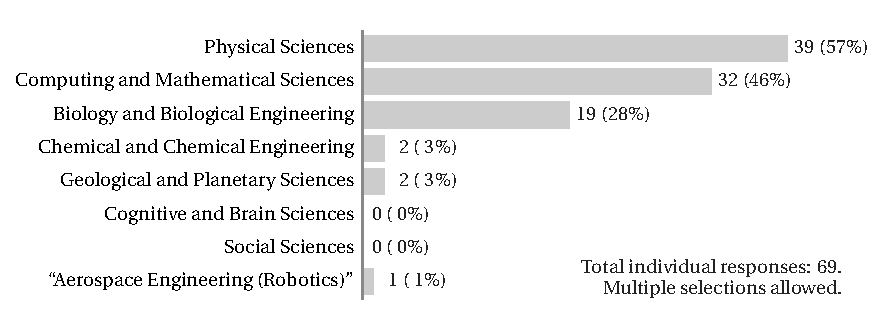
\includegraphics{files/plots/respondents-by-discipline.pdf}
  \vspace*{-3ex}
  \caption{Respondents by discipline.  The survey offered the first eight predefined categories and an additional slot for write-in, free-text answers.  Choices were nonexclusive.  Some respondents included write-in answers but the answers were subsumed by one of the predefined categories; in those cases, we adjusted the totals appropriately.  One response, ``Aerospace Engineering (Robotics)'', did not fit any predefined category; we included it as a true ``Other'' value.}
  \label{disciplines}
\end{figure}

The survey included several questions to gather general demographic information about the respondents.  One of the first questions in the survey was ``What is your primary field of work?'', with multiple choices and ``Other'' as the answer options.  \fig{disciplines} shows the answer choices and the number of responses.  Of \totalrespondents respondents, 57\% identified as working in the physical sciences, 46\% in computing and maths, 28\% in biological sciences and 7\% in a range of others.  Subjects could select more than one field, and respondents made use of this feature: 17 respondents selected two fields of work, six selected three fields, and one indicated four fields of work.

To enable us to gauge how computer-intensive people's work activities are, the survey included the question ``In your work, on a typical day, approximately what fraction of your time involves using or interacting directly with software on a computer or other computing device?''  The answer options were in the form of a pull-down menu with values ranging from 0\% (none) to 100\% (all), in 5\% increments.  \fig{time-with-software} provides a bar graph of the responses.  The results show that the overwhelming majority of our respondents spend over 50\% of their day interacting with software.  To quantify this further, assuming a typical 8~hour working day, we can conclude that 94\% of respondents regularly spent more than four hours of their day engaged with software, and 68\% more than six hours.

\begin{figure}[bht]
  \centering
  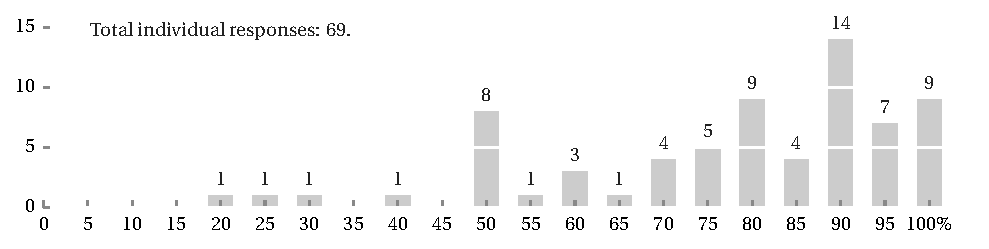
\includegraphics[trim=0.1in 0.1in 0 0,width=6.25in]{files/plots/bar-graph-time-spent-with-software.pdf}
  \caption{Bar graph of responses to the question ``In your work, on a
    typical day, approximately what fraction of your time involves using or
    interacting directly with software on a computer or other computing
    device?''}
  \label{time-with-software}
\end{figure}

As mentioned above, the overall motivation for the survey was to understand how people find software.  Thus, an important precondition was whether subjects actually had a choice in the software they used.  (The rationale for this is that if a person has no choice but to use software that is already provided or selected for them, then their answers to questions about how they find software would not be meaningful.)  This consideration motivated another question in the survey: ``In your work, how much freedom do you usually have to choose the software you use?''.   Answers to this question were used to select subsequent survey questions: if a respondent answered ``Never'' to this question, then the remaining questions were skipped and they were shown the final survey feedback page.  \fig{freedom} provides the results for this question.  It shows that every one of our respondents had some choice in the software they, and consequently all \totalrespondents respondents were shown the next set of questions in the survey.  %In all, 88\% of respondents said that they had \emph{some} degree of freedom to choose the software they used.

\begin{figure}[htb]
  \vspace*{-1ex}
  \centering
  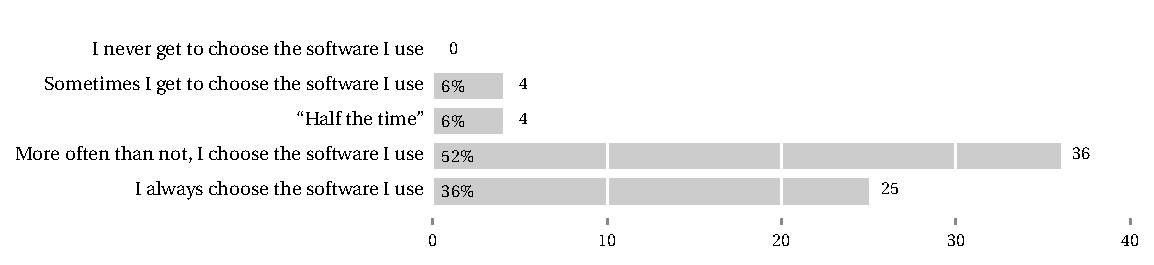
\includegraphics[width=6in]{files/plots/how-often-choose-software.pdf}
  \vspace*{-4ex}
  \caption{Responses to ``In your work, how much freedom do you usually have to choose the software you use?''.}
  \label{freedom}
\end{figure}

In response to another question, ``Are you involved in software development?'', \totaldevelopers (81\%) answered ``Yes'' and 13 (19\%) answered ``No''.  The answer to this question controlled the display of an additional set of questions relevant to developers.  Among the questions that were made available to the \totaldevelopers who answered ``Yes'' were additional demographic questions.  (Those who answered ``No'' were not shown these additional demographic questions or the questions relevant to developers, and were instead taken to the final survey feedback page.  This happened to 13 respondents.)  The first developer-related demographic question was ``For how many years have you been developing software?'' with a free-form text field for answers.  We manually processed the \totaldevelopers text responses to remove extraneous text and reduce them to numbers, and then tabulated the values.  \fig{years} provides a histogram of the responses received for those who answered the question with a usable answer (55 out of \totaldevelopers).

% Note about the data cleaning:
% - if someone wrote "x+" or "at least x", I counted it as x.
% - if someone wrote "~x", I counted it as x.
% - one person wrote "depends on who you ask". I deleted that result.

\begin{figure}[thb]
  \vspace*{1ex}
  \hspace*{0.25in}
  \begin{minipage}[b]{0.3\linewidth}
    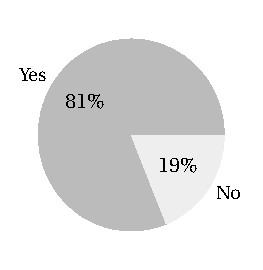
\includegraphics[width=1.5in]{files/plots/number-of-developers.pdf}
  \end{minipage}%
  \begin{minipage}[b]{0.75\linewidth}
    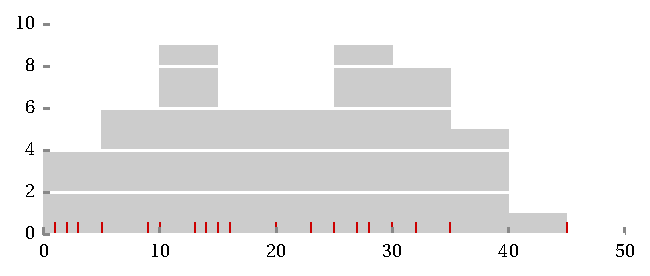
\includegraphics[width=3.7in]{files/plots/histogram-years.pdf}
  \end{minipage}%
  \vspace*{-2ex}
  \caption{(Left) Responses to the question  ``Are you involved in software development?'' (Right) Histogram and rug plot of years that respondents have been developing software (for those who also answered ``Yes'' to the question of whether they were involved in software development).}
  \label{years}
\end{figure}

Another question asked of those who indicated they were involved in software development was ``In your current (or most recent) software development project, what is (or was) your primary responsibility?'' The answers were in the form of eight multiple choice items and a ninth ``Other'' choice with a free-form text field.  The choices were nonexclusive: although we asked for people's primary responsibility, respondents were free to choose more than one and the explanatory text for the question indicated ``If it is hard to identify a single one, you can indicate more than one below.''  \fig{responsibilities} provides a tally of the responses.

\begin{figure}[thb]
  \vspace*{-1ex}
  \centering
  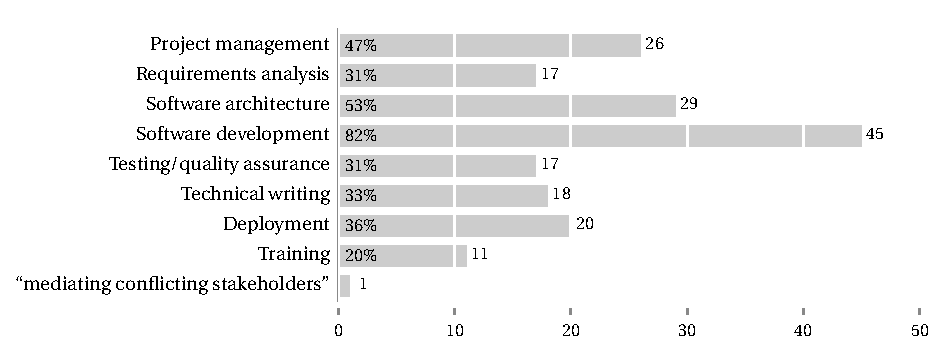
\includegraphics[width=5.9in]{files/plots/responsibilities.pdf}
  \vspace*{-3ex}
  \caption{Responses to the question  ``In your current (or most recent) software development project, what is (or was) your primary responsibility?''  This question was shown only to the 56 respondents who answered ``Yes'' to the question of whether they were involved in software development.  This survey question offered the first eight predefined categories and an additional slot for free text under ``Other''; only one respondent provide a value for ``Other''.  Choices were nonexclusive.}
  \label{responsibilities}
\end{figure}

We also asked, ``What is the typical team size of projects you are involved with?''  The form of the answers was again a set of multiple choice click boxes with an ``Other'' choice that offered a free-form text field.  Answers were provided by all \totaldevelopers respondents who answered ``Yes'' to the question of whether they were involved in software development, and none of the respondents selected ``Other''.  \fig{project-sizes} provides a summary of the results.

\begin{figure}[htb]
  \centering
  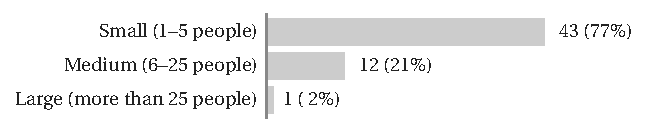
\includegraphics{files/plots/project-sizes.pdf}
  \vspace*{-3ex}
  \caption{Project sizes reported by the \totaldevelopers respondents who indicated they were involved in software development.}
  \label{project-sizes}
\end{figure}

In the final demographic question, we asked ``Which programming and/or scripting language(s) have you had the most experience with?''  This question provided 22 predefined language choices as multiple choices along with a free-text ``Other'' option.  Choices were nonexclusive, and the elaboration under the question explicitly requested ``Please select up to 3 languages which you have used the most''.   The top five responses were: Python (selected by 59\% of respondents), C (50\%), Java (34\%), shell scripting (32\%), and C++ (27\%).

These responses are consistent with expectations for the targeted scientific communities.  We expected to reach computer literate individuals, and due to the distribution channels we used, most likely reached those working in research environments.  Languages such as Python and Java are very popular in those settings, and our survey's numbers for languages are consistent those of a recent Stack~Overflow survey~\cite{stackexchange2016survey} for ``most popular technologies per dev type'' for their respondents who chose ``Math \& Data''.  Most respondents indicated they are involved in software development, and typical development team sizes were small, with 77\% being in groups of 1 to 5 persons.  This is common in scientific software development, and the fact that many respondents indicated they had multiple roles is also consistent---small teams generally require members to take on more than one role.

Amongst the 81\% of respondents who subsequently indicated that they were involved in software development to some degree (and not just end users), the median number of years of software development experience was 20. This also suggests that the typical respondent is mid-career or part of the pre-mobile device computing generation. In addition to software development per se, 65\% indicated that they were also primarily responsible for project management or software architecture, which are traditionally more senior roles.  The demographic data may thus indicate a possible bias in responses against more junior members of the respective communities, such as students and postdocs.  This is of concern because junior members may have different search criteria and development experiences than their more experienced colleagues. This possibility should be borne in mind when interpreting the survey results. The cause of this distribution is unknown.  We speculate that it may be the result of a degree of self selection, in that more experienced individuals are more likely to participate in community surveys.  In any case, the possible experience bias is something that we should aim to redress in future similar efforts.


\section{Results: how respondents find software}

Numbers in parentheses in this section indicate the relative rankings or levels of importance (essential and above-average) given in the survey.


\subsection{Ready-to-use software}
 
We first consider the search for software to use for a particular task rather for development purposes. This does not necessarily imply searching for source code, and our questions emphasized that ``ready-to-run'' was the primary goal.  Note it is plausible that source code availability is a consideration even in this circumstance, and in the second question below, we sought to expose how important this criterion is.

 
\subsubsection{Approaches}
\label{approaches-ready-to-use}

To assess how people located or discovered ready-to-run software, we  asked ``When you need to find ready-to-run software for a particular task, how do you go about finding software?''  The question provided multiple nonexclusive answer choices together with a free-text ``Other'' option.  The specific, predefined answer options were developed based on our own experiences as well as the similar questions posed in other surveys~\cite{sim_2011, bajrachary_2009, linstead_2009} and the results of our pilot run.  Respondents were free to choose more than one answer.  \fig{how-find-ready-to-run} summarizes the results.

\begin{figure}[htb]
  \centering
  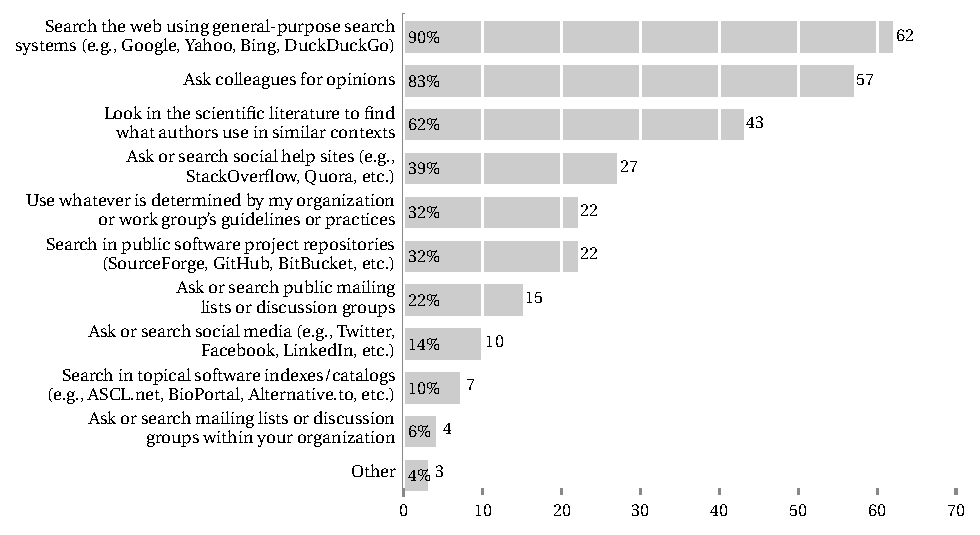
\includegraphics[trim=0.1in 0.1in 0 0,width=6in]{files/plots/how-find-ready-to-run.pdf}
  \vspace*{-1ex}
  \caption{Responses to the question ``When you need to find ready-to-run software for a particular task, how do you go about finding software?'' Answer choices were nonexclusive. All \totalrespondents survey participants answered the question.}
  \label{how-find-ready-to-run}
\end{figure}

Personal recommendations (83\%) and general search engines (90\%) are the two main mechanisms employed to find software by our respondents. If a similar task is also described in the literature, then this will be used as a guide (62\%) to identify relevant software to use. Online forums, whether general social media sites or more focused in scope, are an underutilized resources (mean of 21\%), although people are slightly more likely to search in a public software project repository (32\%) but not in a domain specific one (10\%). This latter usage pattern may reflect ignorance of the existence of the topical indexes in question, but may also reflect a belief that such resources are too narrowly focused in scope for their needs.  The question did not address the size of the task being searched for so we cannot answer this for sure.

The write-in answers for ``Other'' revealed a category of options we did not anticipate: all of the answers concerned the use of network-based software package installation systems such as MacPorts~\cite{fuller2002macports} and the systems available for the different Linux operating system distributions.  In retrospect, this is an obvious oversight in our list of predefined categories---the package management systems offer search capabilities, and thus, this is indeed another way for a person to find ready-to-run software.  Future versions of this survey should include this as a predefined answer choice.


\subsubsection{Criteria}
\label{criteria-ready-to-use}

We sought to understand the selection and evaluation criteria that may come into play when users try to find ready-to-run software.  We posed the question ``In general, how important are the following characteristics when you are searching for ready-to-run software for a task?''  For the answer options, we provided a two-dimensional grid with different predefined criteria as the rows, and values on a unipolar rating scale for the columns.  The available values on the scale were ``Rarely or never important'', ``Somewhat or occasionally important'', ``Average importance'', ``Usually of above-average importance'', and ``Essential''. \fig{criteria-ready-to-run} summarizes the results.  The rows of the bar graph are sorted using sum of ratings for ``Essential'' and ``Usually of above-average importance'' for each criterion, to reveal the most robust trends in the ratings.  Not all respondents provided a value for every criterion in the table, which may be due either to oversight (e.g., if they did not notice they missed a row in the grid) or confusion about the instructions (if they thought they should only rate the ones they cared about).

\begin{figure}[bht]
  \vspace*{-1ex}
  \centering
  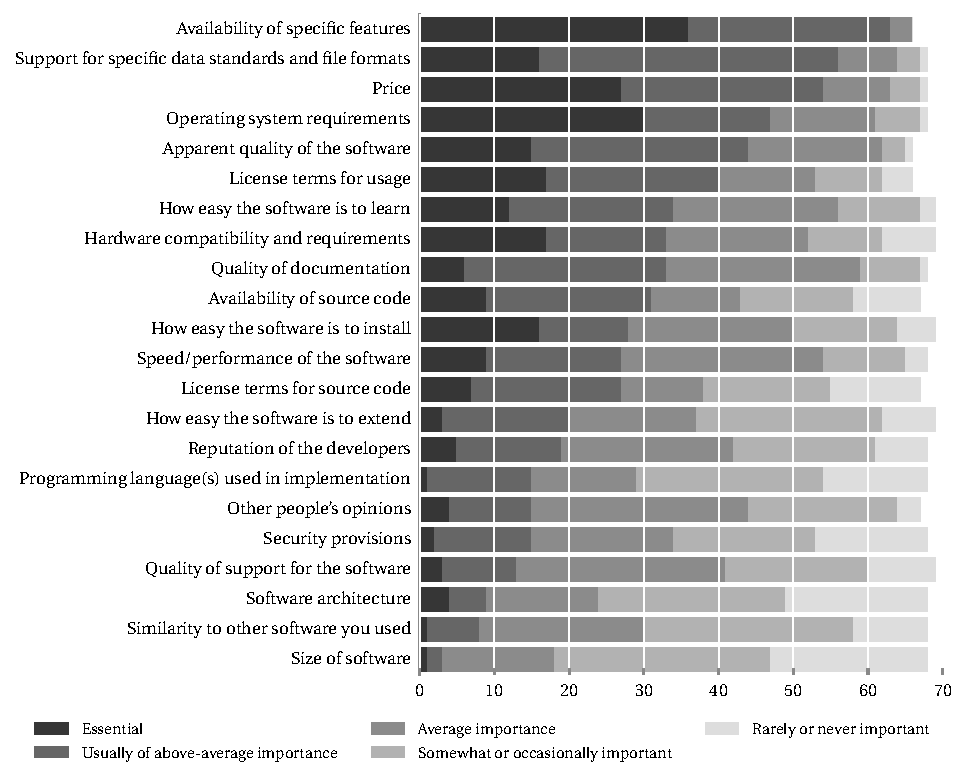
\includegraphics[width=6.2in]{files/plots/bar-graph-criteria-ready-to-run.pdf}
  \vspace*{-2ex}
  \caption{Responses to the question ``In general, how important are the following characteristics when you are searching for ready-to-run software for a task?''  All \totalrespondents respondents answered the question, but not all respondents chose to select an option for every possible characteristic.  The bar graph is sorted by the sum of the number of times the options ``Essential'' and ``Usually of above-average importance'' were selected for each characteristic.}
  \label{criteria-ready-to-run}
\end{figure}

% 2016-02-01 <mhucka@caltech.edu> In the paragraph below, I took out the part about "biological computing tends more towards the use of Windows-based systems" because my experience and that of other people I've asked is that biology is skewed towards Macs and not Windows.  But we don't need to say either way for the point to be made below, so what if we just don't mention it?  

Unsurprisingly, people reported that the primary search criterion is the availability of specific features (95\%) in the software. Support for specific data standards and file formats (82\%) and software price (81\%) are also major considerations, which may reflect the culture of scientific computing---software often is expected to be free, and specific areas of science often use specialized data formats (e.g, FITS in astronomy). Platform requirements, in terms of both operating system (69\%) and hardware (47\%), score more highly than either ease of usage (50\%), installation (40\%) or any performance metrics (39\%). How the software was actually implemented in terms of programming language (23\%) or a particular software architecture (14\%) are unimportant, though.  We hypothesize that this is related to the dominance of particular computing configurations within specific sciences; for example, astronomical computing happens predominantly on Apple or Linux systems.  In that context, if one is searching for software to run, a more pressing constraint may be simply be whether it is compatible with the operating platform rather than how it was written.

Quality and support aspects of the software are secondary considerations as far as software search is concerned, with documentation (48\%) rating higher than either the reputation of the developer (27\%) or the level of software support (18\%).  This suggests that once the software is installed, users expect that they can find in-house workarounds for any bugs, and that they are less concerned about future software updates. This illustrates how scientific computing is different from both commercial computing, where software licenses are purchased with implied support, and mobile computing, where software updates are automatically pushed out to devices.

A more surprising result is that other people's opinions of the software (23\%) and its similarity to other software (12\%) are not important search criteria when they are so important as search mechanisms (see above). It is possible that a search for software is only necessary when there are no word-of-mouth recommendations or literature recipes for particular tasks. In those cases, the approval rating of the software or its apparent familiarity may be largely ignored in favor of other criteria.  Future surveys or interviews could investigate these points more deeply.

Another surprising result is that, even though the question explicitly concerned ready-to-use software, the availability of the source code (46\%) and its licensing (41\%) were still rated as relatively important considerations. This may be the effect of a survey bias, given the large fraction of respondees who identified as developers. Such users are more likely to be willing to---and capable of---altering the software to meet their specific requirements, and the search criteria address this need.

It is interesting to compare these results with those of software engineering studies on desirable traits for successful software projects~\cite[e.g.,][]{subramaniam2009determinants, crowston2003defining, sen2012open}. Intuitively, we expect the criteria would align: the features that people say they use to discriminate between choices when looking for software are presumably the same that distinguish successful software efforts from unsuccessful ones.  It does turn out that code quality, documentation quality, price, and licensing terms are recognized indicators of success~\cite{subramaniam2009determinants, crowston2003defining}; however, our survey respondents were relatively unconcerned with developers' reputations or other people's opinions of software, which does not match expectations.


\subsubsection{Search case histories}

To explore more deeply the topic of how users find software, we sought examples of respondents' past experiences by asking the open-ended question ``(Optional) Please describe a past scenario when you looked for ready-to-run software.''  The survey form provided a text editing field where respondents could write their responses in free-form text.  We received a total of 23 responses, of which 14 contained substantial details about the procedures or steps followed.  \fig{sample-responses} provides three examples taken from among those 14 responses.

\begin{figure}[t]
  \small
  \centering
  \fcolorbox{lightgray}{white}{\begin{minipage}{5.5in}
    \begin{center}
      --- Sample A ---
    \end{center}
    "Looked for a free UML modeler\\
    Googling for some sofware comparison pages\\
    Tried a few one (free or with demo license)\\
    Kept ArgoULM\\
    Not really happy with it"
  \end{minipage}}\\[-0.5ex]
  \vspace*{1.5ex}
  \fcolorbox{lightgray}{white}{\begin{minipage}{5.5in}
    \begin{center}
      --- Sample B ---
    \end{center}
"Recently I needed to find a package that would let me generate uuids in a specific language.  I wanted this to be simple (it wasn't the main point of the project, so I didn't want to reinvent-the-wheel), it ideally needed to be cross platform (testing on mac, running at scale on linux), and it needed to be something that I could install relatively quickly.\\

One large constraint was I needed to find a package that worked even on relatively out-of-date systems. This meant the newer system-packaged libraries weren't available, and trying to build them from source wasn't all that tractable (I quickly was going down a rabbit hole of other dependencies which weren't available on this old system).  So it was very difficult to find a relatively self-contained, especially when I didn't have root access.\\

My approach was to first check with package managers.  That wasn't terribly helpful, without having root access.  My next attempt was to find what would have been included on a new system (found through Googling, StackOverflow posts, man pages, etc). Then finally, I had to start searching for older versions, which were more standalone.  This final process of searching for older packages was much more random-walk googling + trial-and-error.  This last stage was probably the biggest pain.\\

(Ultimately I was able to find some software that did what I needed.)"  \end{minipage}}\\
  \vspace*{1.5ex}
  \fcolorbox{lightgray}{white}{\begin{minipage}{5.5in}
    \begin{center}
      --- Sample C ---
    \end{center}
"Looking for an authorization management software (not authentication).\\
I did some online search, plus got some info from a conference and colleagues developing one.\\
The search went on by some specific requirement about the authorization data model used by software and the interfaces available to the authorization data base.\\
Still no exact solution found.\\
One software was too complex with respect with the tasks we need and seemed to miss a top requirement (still investigating).\\
Another seems simpler but definitely lacks documentation on how to start using it."
  \end{minipage}}
  \caption{Samples of responses received to the question ``(Optional) Please describe a past scenario when you looked for ready-to-run software.''  A total of 23 survey respondents answered this question.}
  \label{sample-responses}
\end{figure}  

Analysis of all responses to this question showed that the tasks covered a wide range of applications, ranging from authorization management software to MCMC samplers to visualization packages. However, the actual process described by different people was often essentially the same: firstly a broad search, usually using Google, with three to four keywords relating to functionality, implementation, and particular formats or standards, if required: e.g. "fits viewer windows" or "grib format Linux". Recommendations from colleagues can also replace the initial broad search phase. The results were reviewed on the basis of the brief descriptions returned and if one obviously met the search context then the link was followed. A typical search would follow four to five such links and subsequent review criteria were then used to compare these. More recent software is definitely favored but many final decisions are only made when different packages have been installed and compared at a functional or operational level: "I like to develop my own critical view by testing extensively the software".

This anecdotal evidence is consistent with the responses to the other questions in our survey. Online searches (for ready-to-use software) are primarily used to identify an initial set of candidate packages that meet a particular set of broad criteria for subsequent (offline) evaluation rather than resulting in the trusted identification of a specific match to a sophisticated query. Although this may reflect user bias, it also points to a lack of functionality in general search engines: one respondent wrote "I really miss freshmeat.net [\emph{a now-defunct software index}] because it allowed you to search for software with particular tags/keywords with particular license and language requirements. I haven't seen a good replacement for that."

Interestingly, the reputation of the organization producing the software can result in a level of trust in the search results: "Saw the first match ... [and] trusted it because their employees and contractors are a large portion of the folks worldwide who work with that data format." The final match also does not have to be a perfect solution, as indicated by comments made in the case descriptions such as "not really happy with it" to "works well enough". This suggests a degree of pragmatism that workarounds will be found for minor issues with the identified software (see above).


\subsection{Source code}

We now the consider the search for software source code.  As described in \sec{demographics}, our survey included the question ``Are you involved in software development?'' Responses were used to control whether the survey system showed additional questions related to software development.  One of those questions was ``How often do you search online for software source code?'' with six answer choices that included ``Never''.  If respondents chose any option other than ``Never'', they were shown additional questions related to searching for source code.  In this section, we discuss the results of that part of the survey.


\subsubsection{Motivations}

Out of the overall \totalrespondents respondents, \totalsearchers (80\%) of them indicated they searched for source code at least some of the time.  \fig{how-often-search-for-src} summarizes the responses received to the question ``How often do you search online for software source code?''  To help understand the motivations for why people search for software, we also asked the question ``What are some reasons why you look for source code (when you do look)?''  Similar to other questions in the survey, it included multiple nonexclusive choices and a free-text ``Other'' field as the answer options.  \fig{why-search-for-src} summarizes the responses.

\begin{figure}[bht]
  \centering
  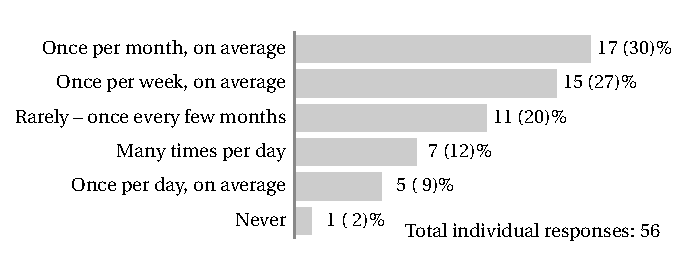
\includegraphics[scale=0.9]{files/plots/bar-graph-how-often-src.pdf}
  \vspace*{-3ex}
  \caption{Responses to the question  ``How often do you search online for software source code?''  Answer choices were presented as the mutually-exclusive multiple choices shown on the vertical axis.}
  \label{how-often-search-for-src}
\end{figure}

\begin{figure}[b]
  \centering
  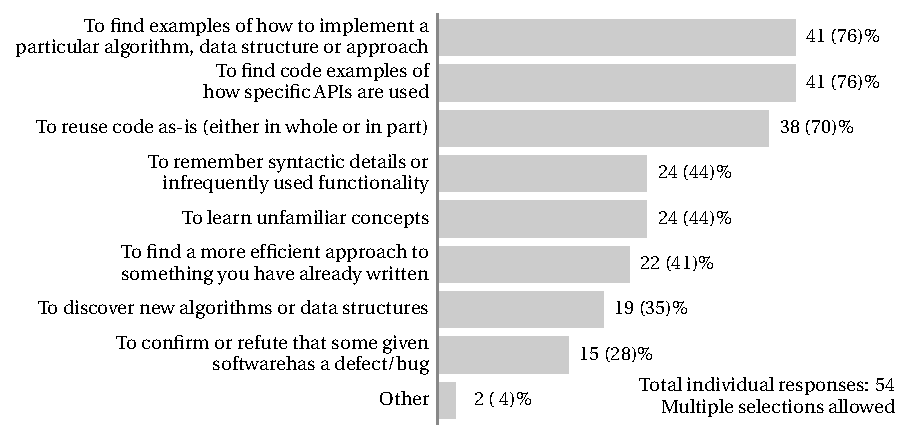
\includegraphics[width=5.6in]{files/plots/bar-graph-why-search-for-src.pdf}
  \vspace*{-2ex}
  \caption{Responses to the question ``What are some reasons why you look for source code (when you do look)?''  This question offered the first eight predefined categories and an additional slot for free text under ``Other''.  Answer choices were nonexclusive.}
  \label{why-search-for-src}
\end{figure}

The results show that our sample of developers typically search online for source code at least once a month (78\%) with some (21\%) searching at least once a day. Coding by example (76\%) or reusing existing code as-is (72\%) are the strongest motivations for searching. This indicates a clear preference for not reinventing the wheel or, at least, a reluctance to start from an absolutely blank slate when developing. Software refactoring is another common reason for searching, either to find a more efficient approach to an existing task (42\%) or to discover new algorithms and data structures (36\%). The web is also used as an online reference source to recall syntactic details (44\%) or learn unfamiliar concepts (46\%). %\note{This is an interesting use case and one we may want to consider further when building interfaces}

Two respondents wrote answers in the ``Other'' field: ``Find software libraries to use'', and ``To understand in detail behaviour of software I'm using''.  Neither are subsumed exactly by other answer options, and indicate additional uses for software source code search that we had not anticipated.  The former answer suggests that examining other developers' code can lead to the discovery of previously unknown software libraries; this is different from searching for how specific APIs are used because it does not presuppose knowing which API library will be found or used.  The second answer suggests that another use of searching for source code is to understand detailed properties of some software, which is different from seeking to reuse code, learning how to use a specific API, or learning about unfamiliar code concepts.


\subsubsection{Approaches}

The survey question ``What are some approaches you have used to look for source code in the past?'' concerned the methods used by developers to find source code.  This question was similar to the earlier question ``When you need to find ready-to-run software for a particular task, how do you go about finding software?''\ but included different answer options that are more relevant to searching for source code.  Answer options were nonexclusive multiple choices, including an ``Other'' option with a field for free-text input.  \fig{how-find-src} provides a summary of the results.  The question was answered by all \totalsearchers respondents who indicated they searched for source code on at least some occasions.

\begin{figure}[thb]
  \centering
  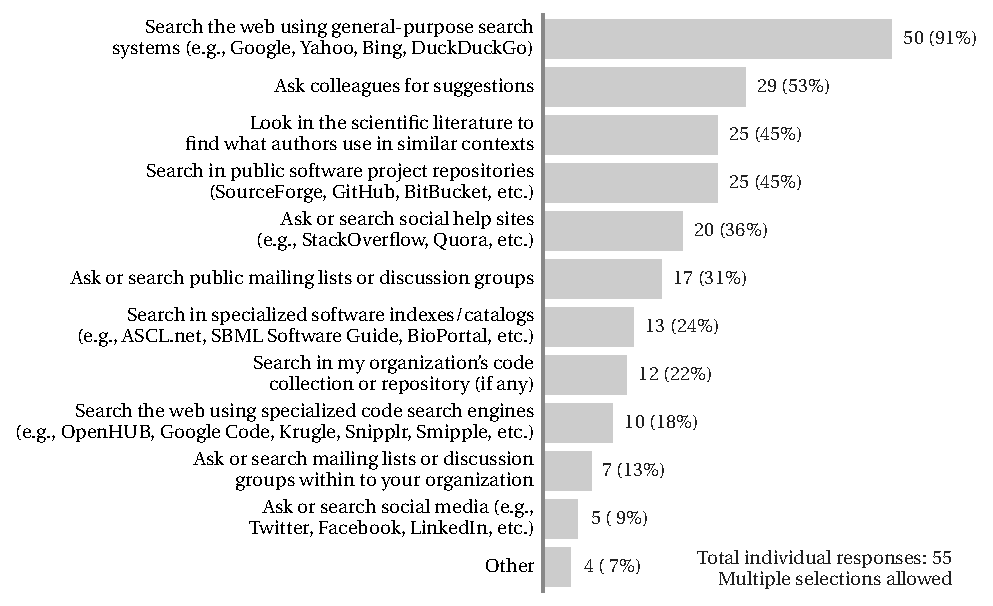
\includegraphics[width=6.2in]{files/plots/how-find-src.pdf}
  \vspace*{-2ex}
  \caption{Responses to the question ``What are some approaches you have used to look for source code in the past?''  This question offered the first eleven predefined categories and an additional slot for free text under ``Other''.  Answer choices were nonexclusive.  A total of \totalsearchers respondents answered this question.}
  \label{how-find-src}
\end{figure}


% FIXME report "other"

General-purpose search engines (91\%) remain the primary mechanism used to search for source code but personal recommendations (54\%) and the scientific literature (45\%) are employed significantly less than when looking for ready-to-use software (\sec{approaches-ready-to-use}). This suggests that software development is a more subjective activity and so source code searches have a more personalized signature, determined in part by personal coding styles. (This may have implications for search anonymity issues.) This view is supported by the two main factors identified for the failure of past code searches (see below): an inability to find any code suitable for purpose (69\%) and a belief that the requirements were too unique (65\%).

The results also indicate that online forums remain underutilized (with a mean of 23\%) but there is slightly greater use of public code repositories (46\%), although not significantly so. Specialized code search engines (19\%) and software indexes (22\%) are also less used than expected but this may again reflect a lack of knowledge of their existence or coverage. It may also be another instance of sample bias with a more mature audience being less likely to use or trust newer domain-specific software, preferring instead more proven general-purpose mechanisms.  24\% cited lack of trust in the options found as the reason for a previous failed search result.


\subsubsection{Reasons for search failures}

The inability to find suitable source code would hinder software reuse.  From our own experiences, we know a search for software can fail for a variety of reasons.  This motivated our inclusion of another question in thes survey, ``What are some factors that have hindered your ability to FIND source code in the past?''  The question included a variety of nonexclusive predefined options, along with an ``Other'' option offering a free-text input field.  The results are summarized in \fig{factors-that-hindered}.

\begin{figure}[htb]
  \centering
  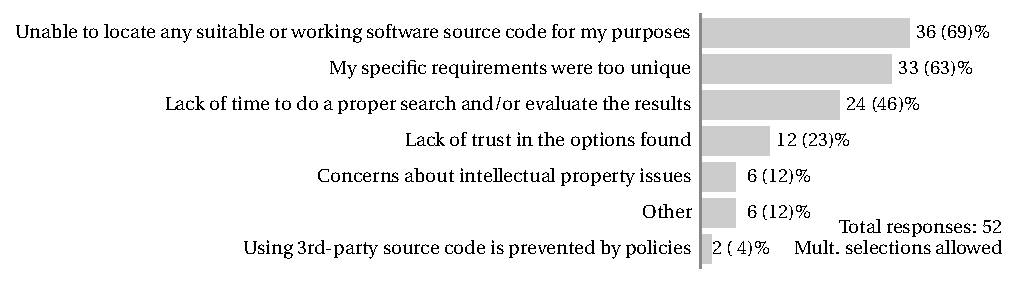
\includegraphics[width=6in]{files/plots/factors-that-hindered-finding-src.pdf}
  \vspace*{-2ex}
  \caption{Responses to the question ``What are some factors that have hindered your ability to FIND source code in the past?''  This question offered the first six predefined categories and an additional slot for free text under ``Other''.  Answer choices were nonexclusive.  A total of 51 survey respondents answered this question.}
  \label{factors-that-hindered}
\end{figure}

There is a reasonable indication (46\%) that time limitations often impact the ability to conduct proper searches for source code or to evaluate the results. This is may be due to the large number of results that general-purpose search engines can return, which in turn may make it difficult to find suitable results easily. This can be particularly the case if the ranking system of the search engine is optimizing a commercial metric, such as potential advertising revenue, rather than metrics more pertinent to searching for software.  The results also suggest that software licensing (12\%) was a minor hindrance to previous successful source code searches, even though it was a relatively important criterion for ready-to-use software (\sec{approaches-ready-to-use}), but it was a large factor (48\%) in not actually reusing the source code found (\sec{reuse-failures}). This suggests that intellectual property information is not sufficiently visible during searches.

% Here are the "Other" answers:
%
% I miss freshmeat.net
% Laziness (didn't try very hard)
% Lack of proper documentation
% I'm not an expert 
% Some scientific software is hidden from search engines as authors did not bother to put it online or make a small website for it.
% Lack of documentation for evaluation of product

The write-in answers for the ``Other'' field provided additional insights into factors that contribute to being unable to locate software.  Six respondents provided ``Other'' answers; three of these were explanatory and useful in this context.  Two respondents cited lack of documentation as a hindrance to either locating or evaluating software.  The third hindrance noted by a respondent was ``Some scientific software is hidden from search engines as authors did not bother to put it online or make a small website for it.''


\subsubsection{Reasons for reuse failures}
\label{reuse-failures}

Being able to find software source code is not the only factor determining whether developers ultimately make use of the code found; other factors can hinder its use.  This motivated our survey question ``If you searched and found source code in the past, what are some factors that may have prevented you from REUSING the source code you found?''  As with most of the other questions in this survey, this one took the form of a multiple choice question with nonexclusive answer options and a free-text ``Other'' field.  We developed the multiple choice options based on our own personal experiences and feedback from the pilot survey.  \fig{hindrance-to-reusing-src} summarizes the results.

\begin{figure}[thb]
  \vspace*{-1ex}
  \centering
  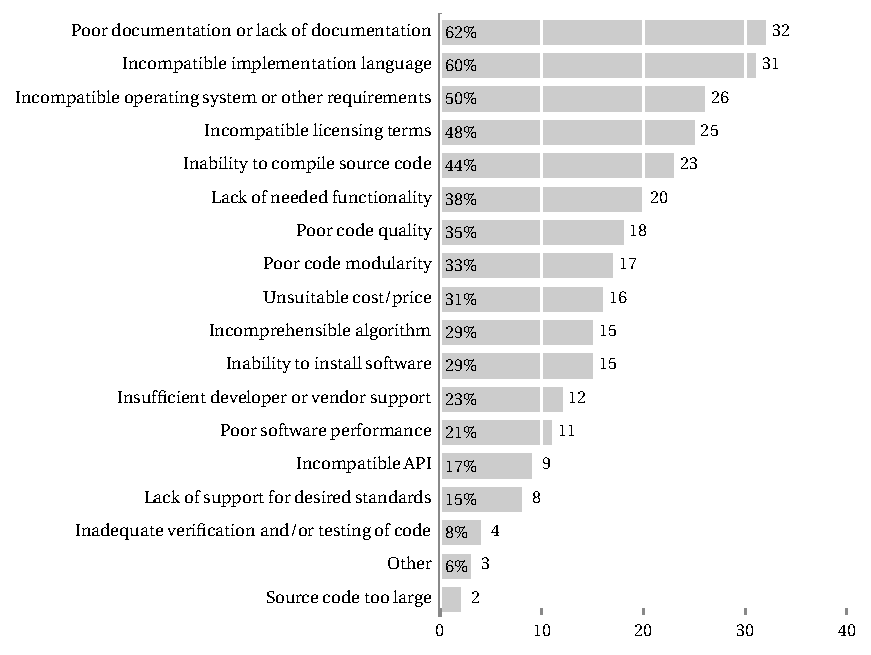
\includegraphics[width=5.65in]{files/plots/hindrance-to-reusing-src.pdf}
  \vspace*{-1.5ex}
  \caption{Responses to the question ``If you searched and found source code in the past, what are some factors that may have prevented you from REUSING the source code you found?''  This question offered the first 17 predefined categories and an additional slot for free text under ``Other''.  Answer choices were nonexclusive.  A total of 52 survey respondents answered this question.}
  \label{hindrance-to-reusing-src}
\end{figure}

The results show that the quality of the documentation (62\%) and implementation details---language (60\%) and operating system (50\%)---are the prime factors in determining whether found software will be reused. An inability to compile (44\%) or install (29\%) the source code also appears to be a relatively common problem, although it is unclear whether this is due to issues with third-party dependencies, compiler versioning, or the actual source code itself.  Other common hindrances are discrepancies between what code purports to do (and so matches a search) and whether it actually \emph{can}: this seems to be more common with functionality (38\%) aspects than support for particular standards (15\%).

The actual quality (35\%) of the code itself, its structure (33\%), and the design of any algorithm (29\%) are less significant factors. Performance (21\%) and verifiability (8\%) are also surprisingly minor considerations to reuse, but this may be related to the didactic nature of many searches: it may not actually be that important if the code is efficient (or even fully functional) if you just want to learn something.

The level of support (23\%) for any code remains a minor factor and pricing (31\%) is also a less significant consideration than for ready-to-run software. Once code has been identified that actually meets the search parameters, it seems that developers are more willing to pay for it (presumably there may be some way to pass the costs on to end-users).


\section{Results: desirable metadata about software}
\label{desirable-metadata}

A potential aid to finding software is a software catalog or index that would classify known software and allow people to browse and search for software by various criteria~\cite{marshall2006software}.  As part of our survey, we sought to determine what kind of information would be important to record about each entry in such an index.  We therefore posed a question of all respondents who indicated they had the freedom to choose software.  (In other words, not only those who indicated they developed software.)  The question was, ``Suppose that it were possible to create a public, searchable catalog or index of software, one that would record information about software of all kinds found anywhere.  What kind of information would you find most useful to include for each entry in such a catalog or index?''  As with most other questions in our survey, we provided answer choices as nonexclusive multiple choices, with an additional free-text option titled ``Other''.  All \totalrespondents respondents to our survey replied to this question.  \fig{info-to-include} summarizes the results.

\begin{figure}[t]
  \centering
  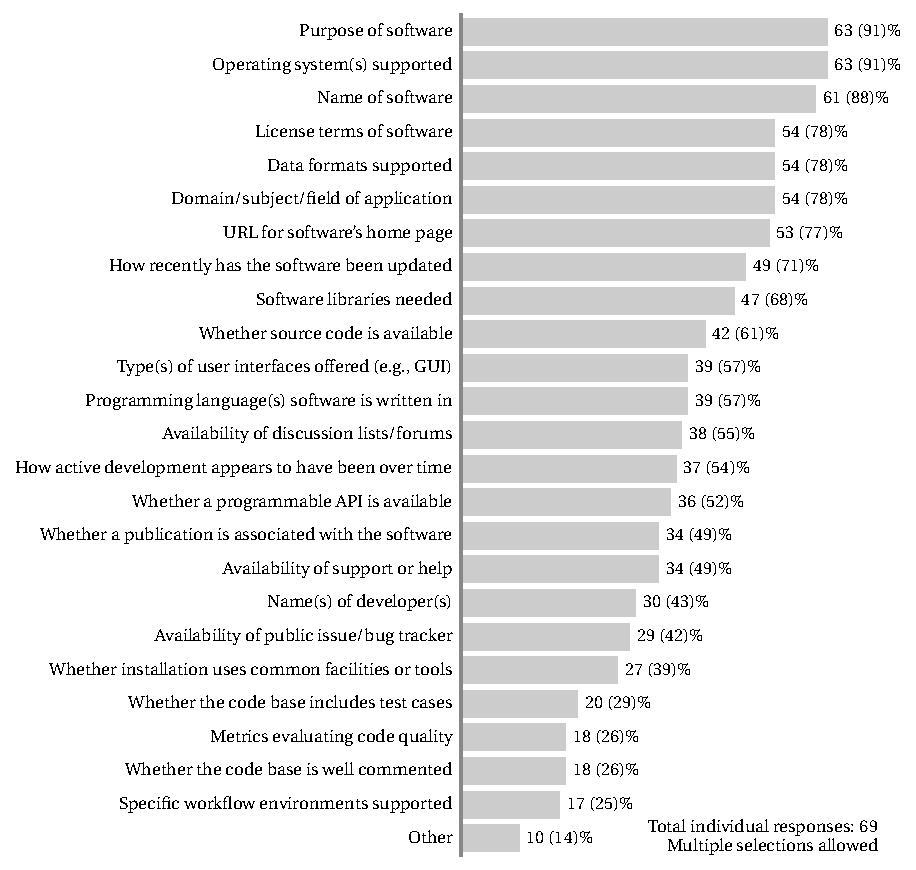
\includegraphics[width=6.1in]{files/plots/info-to-include-in-index.pdf}
  \vspace*{-2ex}
  \caption{Responses to the question ``Suppose that it were possible to create a public, searchable catalog or index of software, one that would record information about software of all kinds found anywhere.  What kind of information would you find most useful to include for each entry in such a catalog or index?'' This question offered the first 24 predefined categories and an additional slot for free text under ``Other''.  Answer choices were nonexclusive.  A total of 69 survey respondents answered this question.}
  \label{info-to-include}
\end{figure}

% Here are the values for "Other":
%   "see also"
%   URL of version control repo
%   size,price
%   whether it is packaged for Debian
%   Documentation!!!
%   Inputs needed (data, parameter format)
%   cost; stability of parent organization
%   Aprrox size of user base
%   Availability of (updated) installation instructions; Availability of plugins (list); Similar tools (list)
%   Size/nature of user base
% 
% I included the "inputs needed" as part of the count of "data formats supported" because it seems like that's what person more or less had in mind.  The rest are unique and discussed below.

The results indicate that simple terms related to functional aspects---the name (88\%), purpose (93\%), domain of application (78\%), data formats supported (76\%)---and operational aspects---operating system(s) (91\%), data licensing (78\%), and dependencies (69\%)---scored most highly. Terms related to an increased degree of sophistication in these areas, such as the types of user interfaces offered (56\%), a programmable API (51\%), or if the installation process made use of common tools (40\%), were ranked less highly.  The availability of documentation, either online (78\%), in online forums (54\%), or in an associated paper (50\%), was also an relatively important criterion, although the availability of support (49\%) or bug tracking (41\%) continue not to be so.

Implementation details, such as the availability of source code (62\%), which language(s) was used (57\%), and the name of the developer (43\%), would be more important to developers. Again, however, more formal aspects---test cases (28\%), well-commented code (26\%) or metrics evaluating code quality (26\%)---rank low. It should be noted that the development status of any code (53\%) and when it was last updated (71\%) rate more highly. This suggests that there is a preference for current software rather than legacy or dead projects, even if they match other search requirements.

Finally, ten individuals wrote additional text in the ``Other'' field of the question.  Analysis of these responses revealed that one answer was similar enough to the predefined categories that we included it in the counts shown in the graph, and one response was not interpretable, but the remaining write-in values constitute sufficiently different categories of information that they are not truly subsumed by any of the options we provided.  The following are the distinct themes that were raised in these responses:

\begin{itemize}[itemsep=-0.5ex]

\item Price (two mentions)
\item Size of the user base (two mentions)
\item Availability of documentation (two mentions)
\item Size of the software
\item Whether it is packaged for Debian
\item URL of version control repository
\item List of plug-ins available
\item List of similar tools
\item Stability of parent organization

\end{itemize}


\section{Results: survey feedback}

In the final question of the survey, we asked respondents to provide feedback on the survey itself.  The 14 comments we received were largely positive, with one or two suggestions about the survey style. Many expressed the opinion that the amount of software available in the world made the construction of a software catalog or index a difficult task but, importantly, that it would a worthwhile endeavor. A few also commented on the broader issue of searching for software, saying that "although [they] do this quite often, [they] never really considered how or why code search succeed or not", and the survey "caused a bit of thinking about issues I rarely consider." One response was more specific on this point: "I wasn't conscious of having explicitly searched for software for a long time. I had to think about it, but turns out I do, quite a lot---but indirectly. I don't search for software---I search for solutions. I search for information about a specific issue, using a fragment from a stack trace, a specific error code, or two or three key words to describe the issue... An indirect reference, such as a one-liner that says 'use xyz to check the status' is more likely to result in a follow up than a whole article written specifically about a product."


\section{Related work}

As part of this project, we performed a lengthy literature survey seeking out research on topics relevant to those in our survey.  We especially sought out other work that may have surveyed how people find or discover software.  We discuss our findings in this section.


\subsection{Surveys examining how software users find ready-to-run software}

Though many surveys have examined software developers and search characteristics in the context of software \emph{code} reuse, extremely few have examined how users---whether they are developers or not---go about locating \emph{ready-to-run} software.  Our research uncovered only three reports of surveys that were not focused specifically on a software development context~\cite{joppa2013troubling, huang2013provenance, lawrence2015science}.

Joppa et al.~\cite{joppa2013troubling} surveyed 596 scientists working in a single domain (biological species distribution modeling), and asked them what software they used and why they chose that particular software.  The reasons given by the respondents provide some insight into how the scientists found the software they used, thus addressing indirectly the same topic as one of our survey questions (see \sec{approaches-ready-to-use}).  In order of most popular to least, the answers that mention something about ``how'' were:
\begin{itemize}[itemsep=-0.5ex]

\item ``I tried lots of software and this is the best'' (18\% of respondents)
\item ``Recommendation from close colleagues'' (18\%)
\item ``Personal recommendation'' (9\%)
\item ``Other'' (9\%)
\item ``Recommendation through a training course'' (7\%)
\item ``Because of a good presentation and/or paper I saw'' (4\%)
\item ``A reviewer suggested I use it'' (1\%)

\end{itemize}

It is interesting to note that none of the responses in Joppa et al.'s~\cite{joppa2013troubling} survey explicitly mentioned searching the Internet via (e.g.)\ a web search engine, although it is possible that some of the answers such as ``I tried lots of software and this is the best'' and ``Other'' subsumed web searches.

Huang et al.~\cite{huang2013provenance} summarized their interviews of 15 students and full-time faculty working in bioinformatics.  They found that four factors influenced the selection of scientific software: (1) suggestions from mentors or senior members of an institution; (2) mentor involvement in the tool's development, in cases where mentors are also developers; (3) the number of publications \emph{about} the software; and (4) the software's reputation, based on the number of publications mentioning the \emph{use} of the tool.  Huang et al.'s report does not include any quantitative or qualitative data about the relative importance of these factors.

Lawrence et al.~\cite{lawrence2015science, lawrence2014who} conducted a large survey in 2014 about the use of science gateways by members of scientific communities.  Their nearly 5000 respondents consisted largely of NSF-funded principal investigators, as well as members of scientific computing centers and others who expressed interest in science gateways.  Several of their questions and results are highly relevant to the topics of our own survey:

\begin{itemize}

\item They asked respondents to indicate domains of expertise, and permitted multiple selections.  The top five were ``Physical and Mathematical Sciences'' (30\%), ``Life Sciences'' (22\%), ``Computer and Information Sciences'' (16\%), ``Engineering'' (16\%), and ``Environmental Sciences'' (14\%), though 16\% did not indicate a domain.  Their top three fields are thus very similar to those chosen by our survey respondents (see \fig{disciplines}), though the proportions are different.

\item They asked how people learn about and choose gateways---a question closely related to our own survey's question about finding software (see \sec{how-find-ready-to-run}).  Their results were that 78\% indicated they learned about technologies from colleagues, 61\% indicated conferences and other meetings as a source, 51\% said publications, 38\% said Web searches and speciality sites, 33\% from students, and less than 10\% from mailing lists or other methods such as magazine advertisements.

\item They asked respondents about the types of Web-based resources were important to their work from the perspective of researchers and/or educators.  The form included a matrix of ten predefined options and 5-term rating scale (``Very important'', ``Somewhat important'', etc.).  The five highest rated resources where: ``Data collections'' (75\% indicated somewhat or very important), ``Data analysis tools, including visualization and mining'' (72\%), ``Computational tools'' (72\%), ``Tools for rapidly publishing and/or finding articles and data'' (69\%), and ``Educational tools'' (67\%).

\item In another question, Lawrence et al.~\cite{lawrence2015science} asked respondents ``Assuming cost is not a factor, what are the most important factors you consider when adopting a new technology? Please select the three (3) most important factors in your decision-making process''.  Since this question had direct relevance to two of our survey's questions (see \fig{criteria-ready-to-run} and \fig{info-to-include}), we include the full response results here:

\begin{itemize}[itemsep=0ex]
\item ``Documentation available'' (49\%)
\item ``Ability to Adapt/Customize'' (35\%)
\item ``Demonstrated Production-Quality Reliability'' (31\%)
\item ``Availability of Technical Support'' (30\%)
\item ``Open Source'' (27\%)
\item ``Existing User Community'' (20\%)
\item ``Interoperability with Other Systems'' (20\%)
\item ``Availability of Support for Bug Fixes \& Requests'' (19\%)
\item ``Testimonials/User Ratings'' (16\%)
\item ``Project Longevity'' (13\%)
\item ``Licensing Requirements'' (12\%)
\item ``Availability of Long-Term Maintenance'' (11\%)
\item ``Reputation of Those Who Built the Software'' (11\%)
\end{itemize}

\end{itemize}

The last outcome summarized above from Lawrence et al.'s survey~\cite{lawrence2015science} is surprisingly different from the results of a similar question in our survey.  Comparing the criteria above to our \fig{criteria-ready-to-run}, neither the relative ordering of the chosen criteria, nor the absolute positions, are consistent between the two sets of survey responses.  The differences are puzzling.  While it is true that our survey included many more possible criteria, and in addition, some criteria in Lawrence et al.'s survey question were coarser in detail, many items in both surveys are comparable, so these two differences alone are unlikely to explain the results.  It is possible that the rankings are influenced by the different answer formats: we asked respondents to rank the importance of each criterion, while Lawrence et al. asked respondents pick their top three criteria.  In an effort to assess whether this is a possible cause, we reanalyzed our results by ranking the responses based on the sum of the number of times ``Essential'', ``Usually of above-average importance'', and ``Average importance'' were selected for each criterion.  The results are shown in \fig{criteria-ready-to-run-reranked}.  Now the quality of documentation is sixth highest in rank, and quality of the software is fourth highest, which begins to approach the high ranks these two criteria had in Lawrence et al.'s survey.  However, other features remain quite different in rankings between the survey results.

\begin{figure}[bht]
  \vspace*{-1ex}
  \centering
  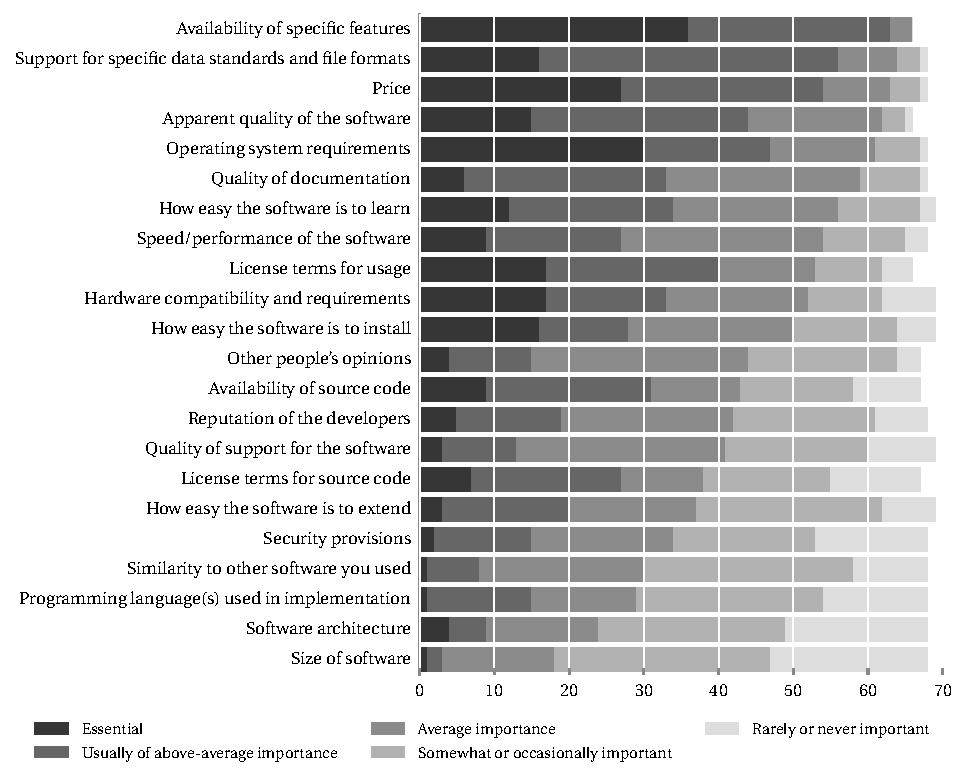
\includegraphics[width=6.1in]{files/plots/bar-graph-criteria-ready-to-run-reranked.pdf}
  \vspace*{-2ex}
  \caption{Reanalysis of the responses to the question of \protect\fig{criteria-ready-to-run}.  In this bar graph, we sorted the possible criteria by the sum of the number of times the options ``Essential'', ``Usually of above-average importance'' and ``Average importance'' were selected for each one.}
  \label{criteria-ready-to-run-reranked}
\end{figure}

Other factors therefore must be responsible for the differences in results between our survey and that of Lawrence et al.~\cite{lawrence2015science}.  We hypothesize two possibilities.  First, the context of their survey was scientific computing gateways, whereas our survey was not focused on this and considered people working with any kind of software environment.  This may influence the criteria people use to select between software options.  Second, Lawrence et al.'s survey had far more respondents than we did.  It is possible that our results for this question would be different if we had more respondents.


\subsection{Surveys examining how developers reuse software}

% It is important to keep in mind that the approaches used by developers in these situations will likely be different from those used by end users to find software, both because developers are known to use different strategies~\cite{} and because are likely to be considering different characteristics (e.g., APIs).  Nevertheless, such studies are related to our survey.

Most studies of how users find software have done so in the context of software development and the reuse of software code.  The types of reuse in these situations range from black-box reuse of libraries or other software components (i.e., reusing code ``as-is''), to reuse of code fragments; in addition, in programming contexts, many studies examined the reuse of other kinds of artifacts such as documentation, specifications, architectural patterns, and more.  For the purposes of this review, we discuss general studies about code reuse in this section, and leave those specifically about code search to the next section.

One of the earliest surveys of software developers in the context of software reuse was published by Frakes and Fox~\cite{frakes1995sixteen}.  In their 1991--1992 survey of 28 U.S. organizations, they received responses to 16 questions from 113 people about questions ranging from programming language and tool preferences to the impact of legal issues.  Several results from this survey are relevant to the topics of our own survey:

\begin{itemize}

\item They found that reuse is more common in some industries than others.  The subjects in Frakes and Fox's study~\cite{frakes1995sixteen} mostly came from high-technology sectors such as the software industry, aerospace and telecommunications.  The authors found significant differences in the reuse of artifacts between different industries, as well as the types of artifacts that were reused.  The telecommunications industry had the highest level of reuse and had the aerospace the lowest.

\item They did not find that having a repository improved reuse.  Frakes and Fox reported that ``organizations with a repository have median code reuse levels 10 percent higher than organizations that do not have reuse repositories, but this difference is not statistically significant at the 0.05 level.''

\item The authors also examined whether company, division or project sizes were predictive of systematic reuse in an organization.  They found no significant correlation between reuse levels and sizes.

\item On the topic of whether respondents prefer to develop their own software versus reusing someone else's, Frakes and Fox found that 72\% of respondents did not have a ``not invented here'' mentality---most developers prefer to reuse when possible.

\item Several of the questions concerned factors that may or may not affect reuse behavior.  We can summarize their results as follows: CASE (Computer Aided Software Engineering) tools do not promote reuse; education about reuse practices improves the level of reuse in an organization; reuse is higher in organizations having a process that promotes reuse;  recognition for practicing reuse does not increase reuse by individuals, but monetary rewards do; and satisfaction with the quality of reusable artifacts did not affect reuse levels among the respondents (but this was because the level of quality they encountered had been adequate).

\end{itemize}

Samadi et al.~\cite{samadi_2004} report preliminary findings from a 2004 survey conducted by the NASA Earth Science Software Reuse Working Group. Their survey was distributed to government employees and contractors in the Earth science community, and asked about people's recent reuse experiences and community needs.  Several results from the study are pertinent to our work:

\begin{itemize}

\item On the topic of how people found reusable software artifacts, the following approaches were noted: (1) word of mouth or personal experiences from past projects, (2) general web search engines (e.g., Google), (3) catalogs and repositories.  The authors report ``Generic search tools (such as Google) were rated as somewhat important, whereas specialist reuse catalogs or repositories were not cited as being particularly important''.

\item As far as criteria used to decide which specific components to choose, the authors report that ``most respondents chose saving time/money and ensuring reliability as their primary drivers for reuse''.  Further, the following additional considerations were noted: (1) ``ease of adaption/integration'', (2) availability of source code'', (3) ``cost of creating/acquiring alternative'', and (4) ``recommendation from a colleague''.  The authors further report that (a) availability of support, (b) standards compliance, and (c) testing/certification, were ``not ranked as particularly important''.

\item On the topic of barriers to reuse, two common types of barriers emerged: (1) if available software did not meet a person's specific requirements, and (2) if a given software artifact was ``difficult to understand or poorly documented''.

\end{itemize}

The same study was reprised in 2005 with a wider audience that included members of academia.  The survey and the results of 100 responses they received are summarized by Marshall et al.~\cite{marshall2006software}.  According to Marshall et al., the larger 2005 survey produced essentially similar results to the preliminary 2004 survey.  The noted the following:

\begin{itemize}

\item The primary reason given by people for not reusing software from outside of their group was that ``they did not know where to look for reusable artifacts and they did not know suitable artifacts existed at the time''.

\item For respondents who did engage in reuse, ``personal knowledge from past projects and word-of-mouth or networking were the primary ways of locating and acquiring software development artifacts.''  

\item On the topic of how people located software, the results reported by Marshall et al.~\cite{marshall2006software} seem to be inconsistent.  The authors noted that ``Web searches were of average importance while serendipity and reuse catalogs or repositories were rated the lowest''; however, in another section of the survey dealing with how to increase reuse within the Earth science community, one of the top three factors was ``having an Earth science catalog/repository for reusable artifacts.''  In other words, catalogs were rated low in one part of the survey but high in another part.  Despite this, among their conclusions, Marshall et al. noted ``the use of reuse catalogs and repositories was rated the most important method of increasing the level of reuse within the community.''

\end{itemize}

In a different NASA-centered study, Orrego and Mundy~\cite{orrego_2007_study} studied software reuse in the context of flight control systems at NASA's Independent Verification \& Validation (IV\&V) Facility.  They studied 63 projects using interviews, surveys and case studies.  In interviews with 15 people, they found that black-box reuse and other types of reuse did occur, and the degree to which a given project reused software ranged from 0\% to 80\%.  The difficulty of assessing the characteristics of software was stated as the most problematic aspect of reusing software, usually because of inadequate documentation for the software components to reused.  Unfortunately, the Orrego and Mundy did not report the specific approaches attempted by people to locate software.

Singer et al.~\cite{singer2014software} examined how software developers active on GitHub use Twitter.  They conducted an initial exploratory survey with 271 users of GitHub users (270 of who said they develop software) and followed it up with a validation survey involving 1,413 GitHub users (1,412 of whom said they develop software).  Their results have the following relevance to the topic of how people find and choose software:

\begin{itemize}

\item Developers increase their awareness of people, trends and practices by subscribing to Twitter accounts by (a) individual developers as well as software project news channels relevant to their work, (b) news services or news curators, (c) ``thought leaders'' or experts in different subject areas.  

\item Developers extend their knowledge of software (including new software tools and components) by asking and answering questions, participating in conversations, and following experts.  This can learn to serendipitous discovery of reusable methods, software components and software tools.  Singer et al. noted ``Some developers mentioned that Twitter helps them find and learn about things that they would not have been able to search for themselves, such as emerging technologies that are too new to appear in web searches.''

\end{itemize}

Bauer et al.~\cite{bauer2014exploratory} describe a study of reuse practices by developers at Google.  Despite the nature of Google as one of the preeminent software organizations today, it is surprising that there is no centrally-controlled mandate about reuse of software.  The question of what to reuse, and how, is left to engineers and managers.  (There are core libraries and software components that get reused company-wide; these are under the care of dedicated teams, but the decision of what to use for a given task or application is evidently up to individuals and product teams.)  Several of the questions in Bauer et al.'s survey~\cite{bauer2014exploratory} are relevant to the present study.

\begin{itemize}

\item They asked subjects for their top three ways of sharing software components.  They received 63 responses: common repository (97\%), packaged libraries (34\%), tutorials (31\%), blogs (19\%), email (9\%), ``I do not share artifacts'' (3\%), and ``other'' (3\%).

\item They asked about the preferred ways to find reusables.  They received 106 responses: code search (77\%), communication with colleagues (64\%), web search (49\%), browsing repositories (41\%), browsing documentation (23\%), ``other'' (8\%), ``code completion'' (5\%), code recommendation systems (3\%), and tutorials (3\%).  It is worth noting that Google has a centralized code repository where most of the code is available for all projects; this system features a centralized code search facility.

\item They also asked, ``What do you do to properly understand and adequately select reusable artifacts'' yielded 115 responses: interface documentation (72\%), examples of usage on blogs and tutorials (64\%), reviewing implementations (64\%), reading guidelines (51\%), exploring third-party products (28\%), ``other'' (10\%), and participating in training for third-party products (5\%).

\end{itemize}

A final study relevant to this topic is the work of Lawrence et al.~\cite{lawrence2015science, lawrence2014who}, discussed in the previous section.  An additional question in their survey is relevant in the context of software search and reuse by developers.  They asked software developers ``How do you keep up to date with web-based technologies'', limiting answers to two choices from a predefined list and a free-text ``Other'' field.  The three most popular answers were using online communities via email or Web-based forums (47\%), one's own development team (43\%), and focused workshops (18\%).


\subsection{Surveys examining code search by developers}

It has been long known from studies of developers at work~\cite[e.g.,][]{singer1997examination} that search is always a common activity.  A number of studies have also examined more specifically how developers use search to discover software.  It is important to keep mind, however, that while they are relevant to the general question of how users find software, such studies presuppose an answer: the users are \emph{performing search} on a computer, and not (say) reading papers or asking colleagues for recommendations.  Thus, the studies have a narrower scope than our survey, both in terms of the populations studied and in terms of approaches to finding software.  On the other hand, they can delve more deeply into the details of how, where, when, and why the subjects searched for software.

Umarji et al.~\cite{umarji_2008, umarji_2013} surveyed Java programmers in 2006--2007 to understand how and why they searched for source code.  They solicited participation to fill out a web survey via invitations to mailing lists and newsgroups, and received 69 responses.  In the 2008 paper and the 2013 book chapter, they focused on one of the survey questions asking people to describe 1--2 scenarios in which they looked for source code on the Internet.  (A similar but earlier study by Sim et al.~\cite{sim_1998} predated the common use of Internet search for code; it has less relevance to the present work, so we do not report on it here.)  Several facets of the Umarji et al. study are especially relevant to our own survey:

\begin{itemize}

\item With respect to why developers searched, out of a total of 51 searchers described, Umarji et al.~\cite{umarji_2008} found that the largest fraction were concerned with finding either (a) reusable code (67\% of the 51 results), (b) reference examples (33\%), or debugging activities (10\%).  Within the reuse category (a), the authors identified four themes: (1) search for code fragments; (2) search for subsystems that implemented reusable data structures, algorithms, or other elements that could be incorporated into an implementation; (3) search for packages or API libraries; and (4) search for stand-alone tools or systems (in the words of a respondent, ``big piece of code that does more or less what I want'').  Within the category of reference examples (b), Umarji at al. also identified four (different) themes: (1) search for code fragments that illustrate syntax; (2) search for implementations of data structure, algorithm or widgets in order to verify a programmer's own approach or use as a basis for reimplementation; (3) search for examples of how to use a library; and (4) search for similar software to generate new ideas.  Within the category of debugging (c), developers searched for solutions to software defects (``patches'') or explanations for the cause of an error.

\item Umarji and Sim~\cite{umarji_2013} report that common starting points for searches were: (1) recommendations from friends, and (2) reviews, articles, blogs and social tagging sites.

\item With respect to how developers conducted searches, the participants in the survey used the following, in order of popularity: (1) general-purpose search engines (87\% of participants), (2) personal domain knowledge (54\%), (3) project hosting sites such as SourceForge.net~\cite{sourceforge_1999} (49\%), (4) references from peers (43\%), (4) mailing lists (23\%), and (5) code-specific search engines such as Google Code Search~\cite{googlecodesearch_2006} (16\%).

\item With respect to the selection criteria used by developers to choose a solution, Umarji and Sim~\cite{umarji_2013} report that the most important factors in order of importance were: (1) functionality (78\%), (2) type of software license (43\%), (3) price (38\%), (4) amount of user support available (30\%), and (5) level of project activity (26\%).

\end{itemize}

Gallardo-Valencia and Sim~\cite{gallardo2011kinds} examined the web search behaviors of 25 developers working at a software company that develops transactional software for banks and other organizations.  The authors used several methods to gather their data: they asked developers to self-report their activities using record sheets, they performed interviews, and they performed observation of developer activities during their work days.  They reported that 8\% of the web searches performed by developers during the study period were to download libraries or other tools, and another 5\% of the web searches were to collect information to help judge the suitability of software components to be used in implementations.  The rest of the searches concerned finding information about how to do specific tasks or write specific kinds of programs, and debugging problems involving errors in software.

Sim et al.~\cite{sim2012software} performed a pair of surveys as part of an effort to understanding developers' approaches to code search.  One survey was exploratory and used to inform a second, quantitative survey.  They report only a small part of the survey results, specifically concerning the nature of the searches performed in the different surveys.  For purposes of the current review, the quantitative survey results are more relevant.  On the topic of what subjects searched for, 92\% of respondents in their survey answered they had searched for code snippets on past occasions, and 69\% said they had searched for software components.  In terms of motivations for why they conducted searches, 96\% of respondents said they had sought reference examples on past occasions, and 35\% said that they had searched for code to reuse as-is.

Sadowski et al.~\cite{sadowski2015developers} surveyed and analyzed search behaviors of 40 software developers at Google, Inc.  To  implement the survey, they developed a Web browser extension that directed developers to a survey system whenever the developers accessed an internal code search system at the company, and asked the survey participants to install this browser extension when they worked.  The survey system asked developers four multiple-choice questions before they started a search.  Sadowski et al.\ also analyzed search logs, but their survey is most pertinent to our efforts.  Two questions are directly related to questions we also asked in our own survey:

\begin{itemize}

\item They investigated why developers searched and what questions they tried to answer with their code search.  The most common theme (33.5\% of the survey responses) dealt with getting specific information about an API library or examples of its use.

\item They also investigated the contexts in which code search is used.  The most common situation (39\% of survey responses) was performing searches while working on a code change during development.  In this context, almost half of the developers (46\%) used code search to understand how code worked.

\end{itemize}


\subsection{Other studies}

In addition to the related surveys reported here, there are other works not reviewed here that have applied other methods to examining developer behavior.  The two main classes of non-survey techniques have been the analysis of search engine logs~\cite{bajrachary_2009, bajracharya2012analyzing, jansen_2006, teevan_2004, brandt2009two, brandt2010example, Li2009751, ge2014developers, volske2015users}, and observational studies (often coupled with interviews), either in institutional settings or in laboratory environments~\cite{sim_2011, brandt2009two, banker1993repository, gallardo2013software, sherif2003barriers, pohthong2001reuse, sim2013controlled, murphyhill2015how, sim2011getting, dabbish_2012}.  Due to the different techniques and intentions behind these efforts, the results are difficult to compare directly to our survey.  Nevertheless, in future work we may seek to analyze them more systematically, with the goal of extracting information about how the subjects proceeded to find software and what features subjects found most useful when selecting between software options.


\section{Conclusions}

Before the advent of the World Wide Web, before even the advent of the current Internet, it was paradoxically easier to find software---there was less of it, and there were simply fewer places to look.  Initially, bulletin boards and archive sites using FTP made software available for copying by anonymous users over telephone networks; the Usenet culture~\cite{emerson1983usenet} of the 1980's encouraged widespread sharing and even devoted a newsgroup (\emph{comp.sources}) to the exchange of software source code.  Fast forward to today, and the staggering wealth of software resources available to users is both a blessing and a curse: one can simultaneously feel that for any given task, ``surely someone has already written software to do this,'' and yet an attempt to find suitable software can seem like falling into a rabbit hole.

% 2016-02-02 <mhucka@caltech.edu> Been thinking about this, and
% since we have non-US people, and we don't know numbers for
% biologists, it seems like safest to just not bring this up:
%
% "Although the survey response was not large\note{how many
% would we consider large? There are 2000 professional
% * <drmjgraham@gmail.com> 2016-02-22T19:49:20.141Z:
%
% ^.
% astronomers in the US and we got ~1\%}, "

So what \emph{do} users do today when they want to find software?  This survey was an attempt to gain insight into the approaches used by scientific users as well as the criteria that people apply to select between alternative software choices.  Our respondents worked primarily in the physical, computing, mathematical and biological sciences; the majority were involved in software development and had a mean of 20 years of experience; most worked in small groups; and all had some degree of choice in the software they used.  The self-selection of respondents and convenience sampling used in our survey means we cannot draw quantitative conclusions about the larger population; however, our survey's results are reasonably similar to those of other past surveys, both in scientific communities and in the broader commercial world where the question topics overlap, and this gives us reason to believe that our results are qualitatively representative of the subcommunities we sampled.

The survey results help identify a number of current community practices in searching for both ready-to-use software and source code:

\begin{enumerate}

\item When searching for ready-to-run software, the top five approaches in order of popularity are: (i) search the web with general-purpose search engines, (ii) ask colleagues, (iii) look in the scientific literature, (iv) look in social help sites such as StackOverflow, and (v) use whatever is determined by the guidelines or work practices of the group or organization where one is working.

\item The top five criteria given above-average weight when searching for ready-to-run software are: (i) availability of specific features, (ii) support for specific data standards and file formats, (iii) price, (iv) operating system requirements, and (v) apparent quality of the software.

\item The top five approaches used by developers to search for source code are almost identical to those used to find ready-to-run software.  They are: (i) search the web with general-purpose search engines, (ii) ask colleagues, (iii) look in the scientific literature, (iv) search in public software project repository sites such as GitHub, and (v) look in social help sites such as StackOverflow.

\item The top five reasons developers search for source code are: (i) to find examples of how specific APIs are used, (ii) to find examples of how to implement something, (iii) to reuse code as-is, (iv) to remember syntactic details or infrequently used functionality, and (v) to learn unfamiliar concepts.

\item The top five reasons developers are unable to reuse the code they find are: (i) poor documentation, (ii) incompatible implementation language, (iii) incompatible operating system or other requirement, (iv) incompatible licensing terms, and (v) inability to compile source code.

\item Finally, we also asked people to indicate the information they would like to see in a software catalog.  A total of 15 features were indicated as desirable by at least 50\% of the respondents, with operating system support, purpose of software, name of software, license terms, and domain/field of application being the most-often requested features.

\end{enumerate}

These have implications for development of catalogs or other resources to help people find software.  

Finally, in this survey, we did not target or exclude scientific gateway communities.  The survey questions generally did not mention gateways or portals explicitly; the closest was the question discussed in \sec{desirable-metadata}, which included workflow environments as an answer choice.  Based on the responses reported in \fig{info-to-include}, 25\% respondents consider support for workflow environments a criterion in selecting software.  Since we did not ask about it explicitly, it is unclear whether any of the respondents had the use of gateways in mind and framed their responses accordingly.  It is also not clear what effect this would have had on their responses.  It is therefore possible that this is a confounding factor in our results: gateways concentrate software resources in one location and typically provide an index or other means of finding software provided by the gateway, and it is conceivable that this may change the nature of how users think of finding software or the criteria they use to discriminate between available alternatives.  Future surveys should make this aspect explicit.


% The breadth and maturity of response has helped to identify a number of current community practices in science in searching for both ready-to-use software and source code. It has also raised a number of issues that need to be considered in the design of a software index or catalog:

% \begin{enumerate}
% \item Searching for reference material vs. production code - pedagogic code may not be efficient.
% \item Personalized search profiles
% \item Result trust issues
% \item Evaluatory statistics 
% \item Licensing metadata
% \item Full-text index matching from READMEs against search strings to identify "one-liners" rather than just keywords
% \end{enumerate}


\section{Acknowledgments}

This work was funded by the USA National Science Foundation, award \#1533792.  


% ......................................................................
\appendix
\section{The Survey}
\label{apdx:survey}

We implemented the survey using Google Forms~\cite{googleforms}, a free online system for creating interactive, Web-based forms.  The following pages show screen captures of the survey as it appeared to users.  Not shown is the switching logic that allowed some parts of the survey to be showed only if users responded in certain ways to some of the questions.  The following are the rules implemented in the switching logic:
\begin{description}

\item \emph{Rule for Question 6}: If the user answers ``I never get to choose the software I use'', the next page shown is the final page of the survey (containing questions~21 and~22).

\item  \emph{Rule for Question 11}: If the user answers ``No'', the next page shown is the final page of the survey.

\item \emph{Rule for Question 16}:  If the user answers ``Never'', the next page shown is the final page of the survey.

\end{description}


\clearpage
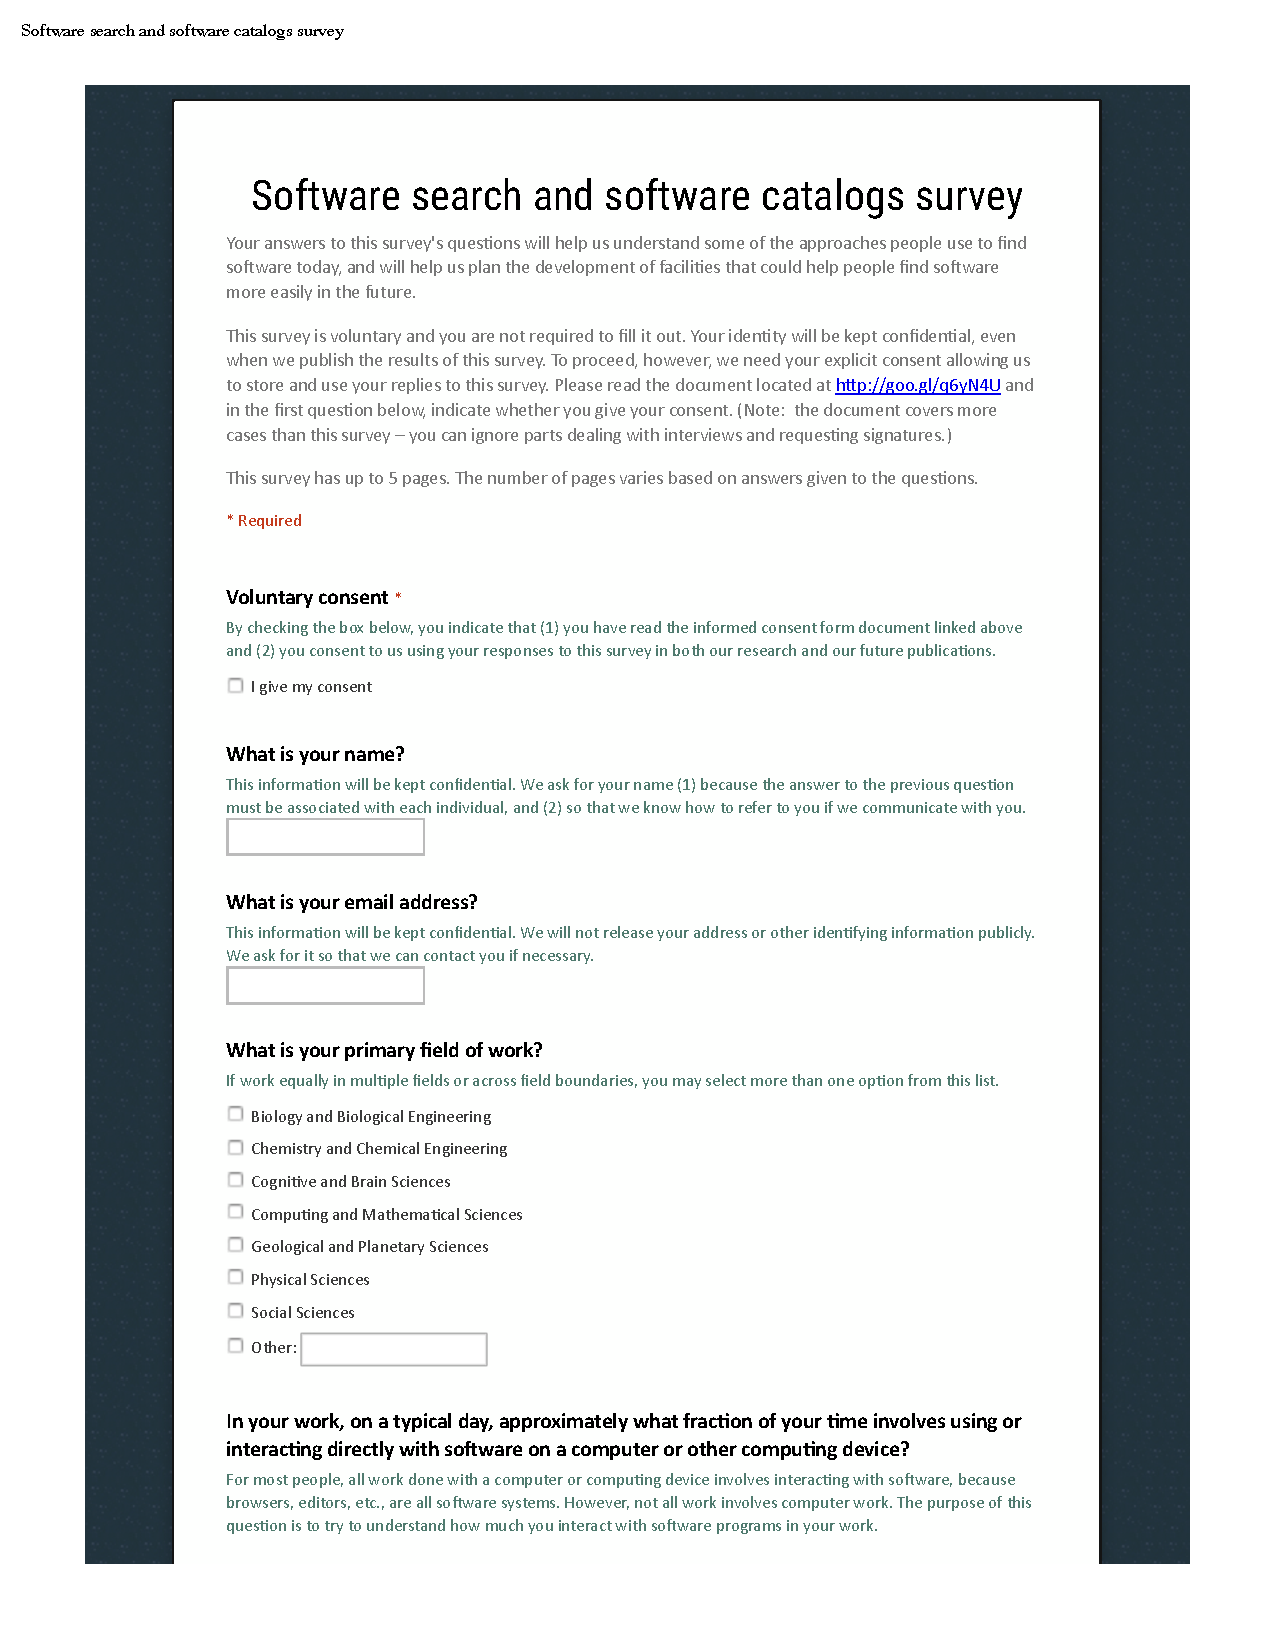
\includepdf[trim=0.25in 0.25in 0.25in 0.3in,pages={-}]{files/survey-copy/survey-2015-09-02.pdf}



% ......................................................................
\clearpage
\bibliographystyle{plain}
\bibliography{mike-casics-library}

\end{document}